\begin{figure}[t]
    \centering
    % First row
    \begin{subfigure}{0.49\textwidth}
        \centering
        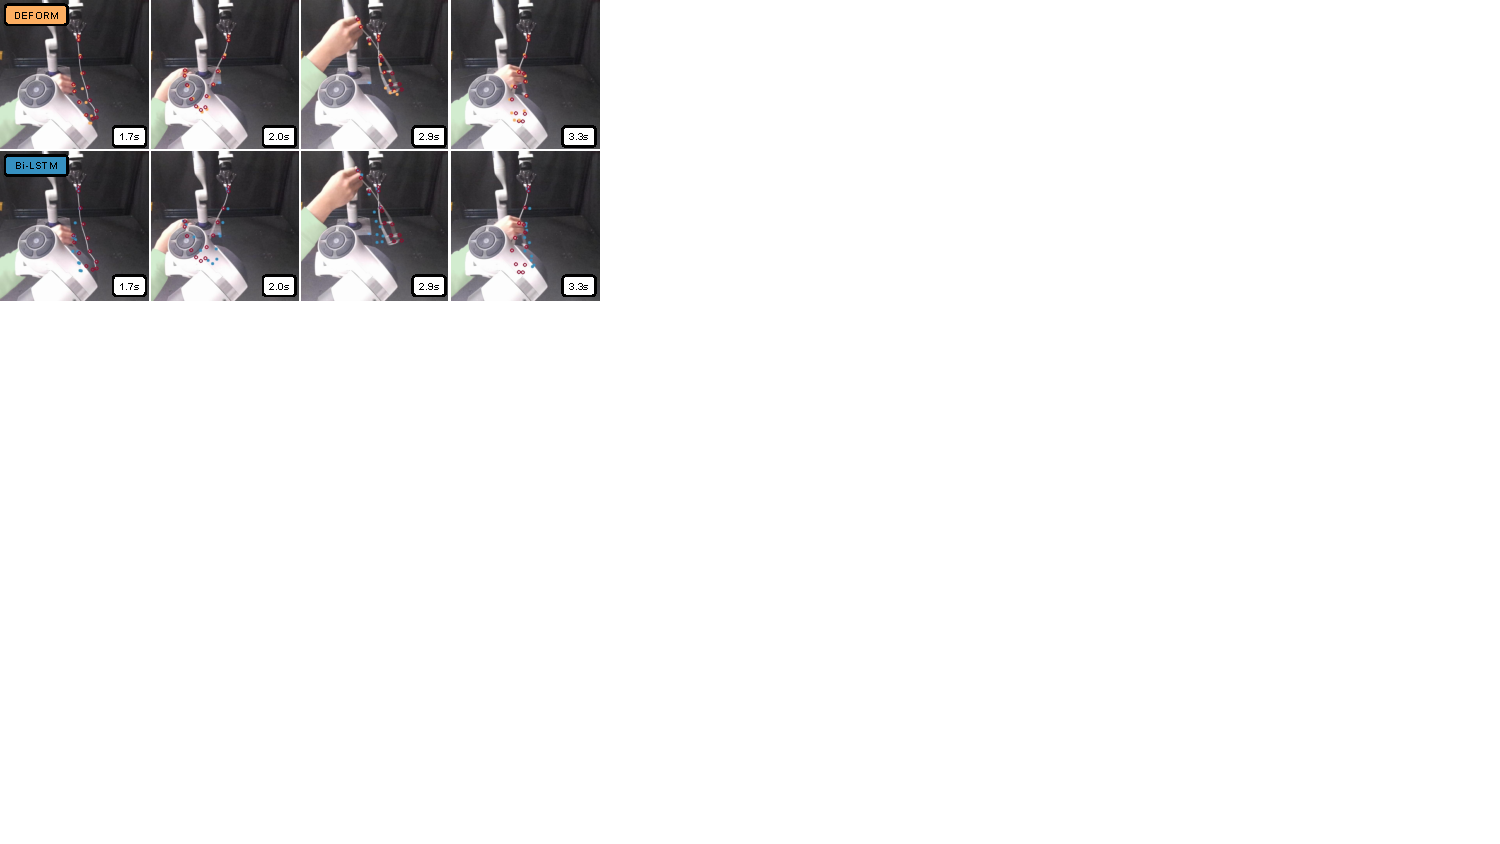
\includegraphics[width=\linewidth]{figures/exp_res_1.pdf}
        \caption{DLO 1, robot-human manipulation}
        \label{fig:rh_thin}
    \end{subfigure}%
    \hfill
    \begin{subfigure}{0.49\textwidth}
        \centering
        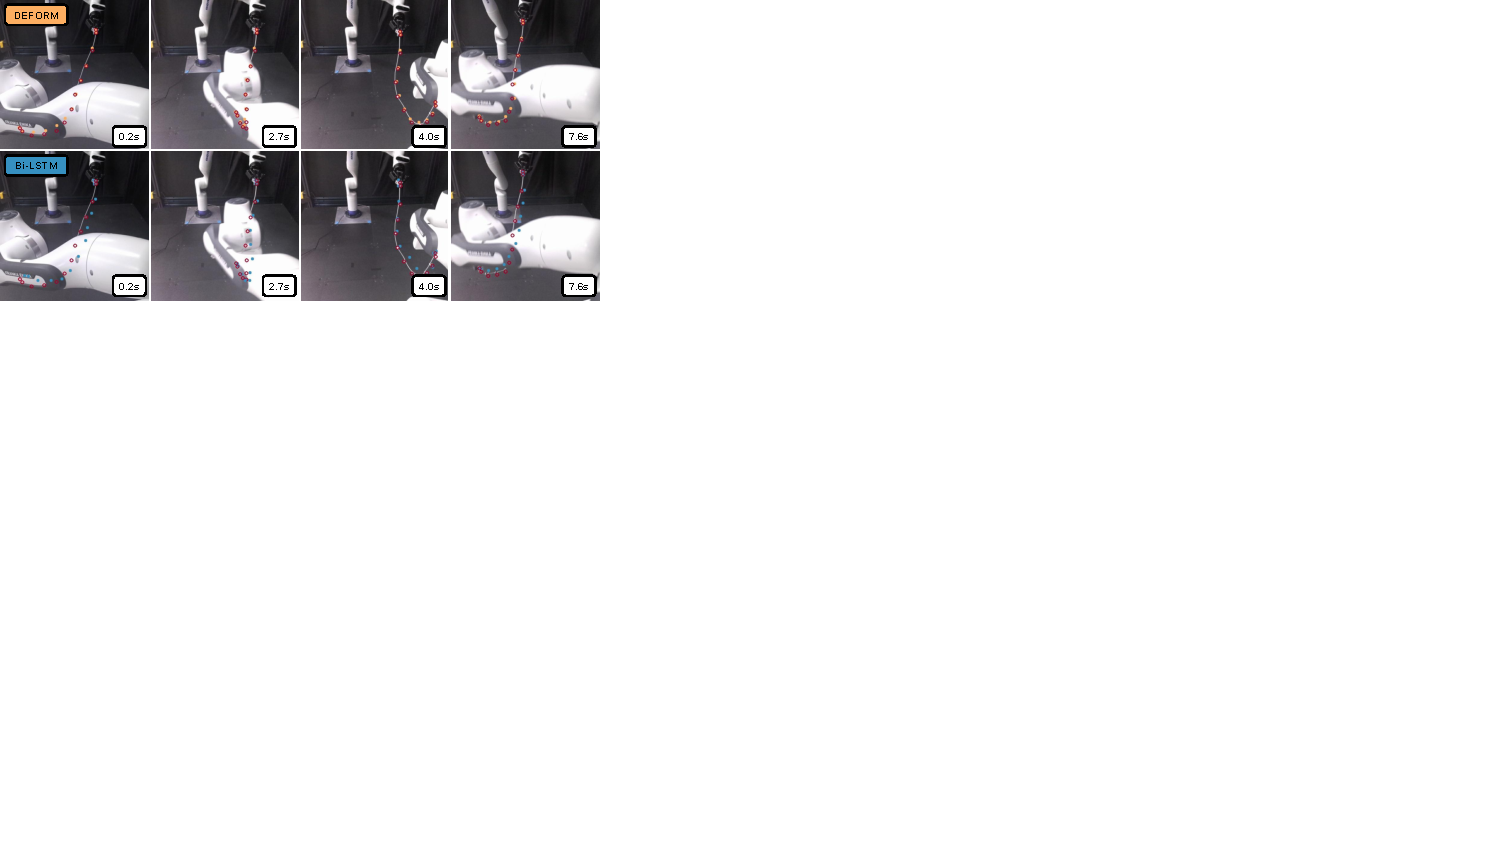
\includegraphics[width=\linewidth]{figures/exp_res_2.pdf}
        \caption{DLO 1, dual-robot manipulation}
        \label{fig:rr_thin}
    \end{subfigure}
    % \vspace{0.18cm}

    % Second row
    \begin{subfigure}{0.49\textwidth}
        \centering
        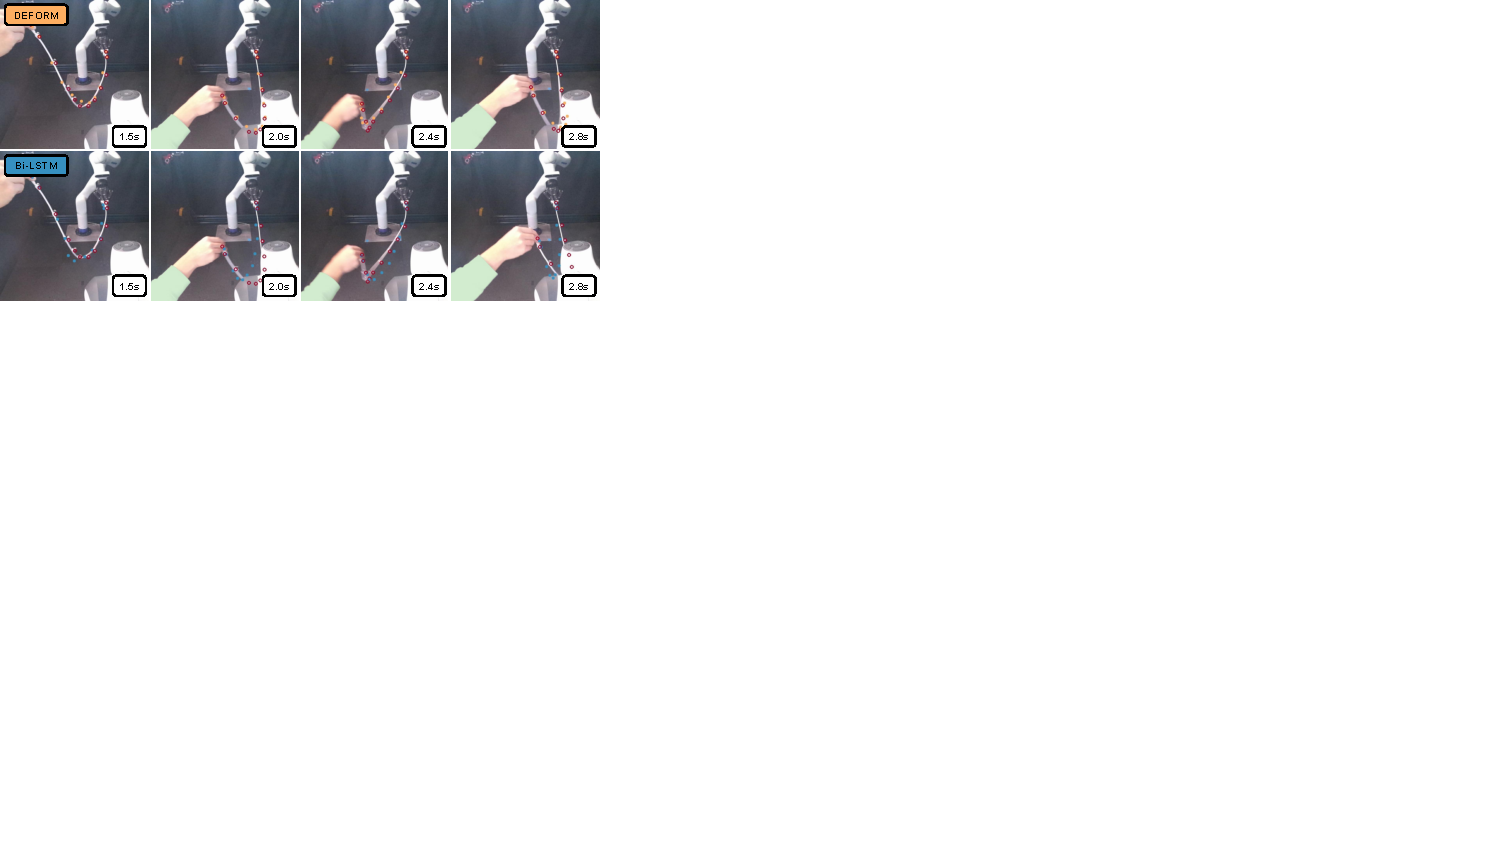
\includegraphics[width=\linewidth]{figures/exp_res_3.pdf}
        \caption{DLO 2, robot-human manipulation}
        \label{fig:rh_thick}
    \end{subfigure}%
    \hfill
    \begin{subfigure}{0.49\textwidth}
        \centering
        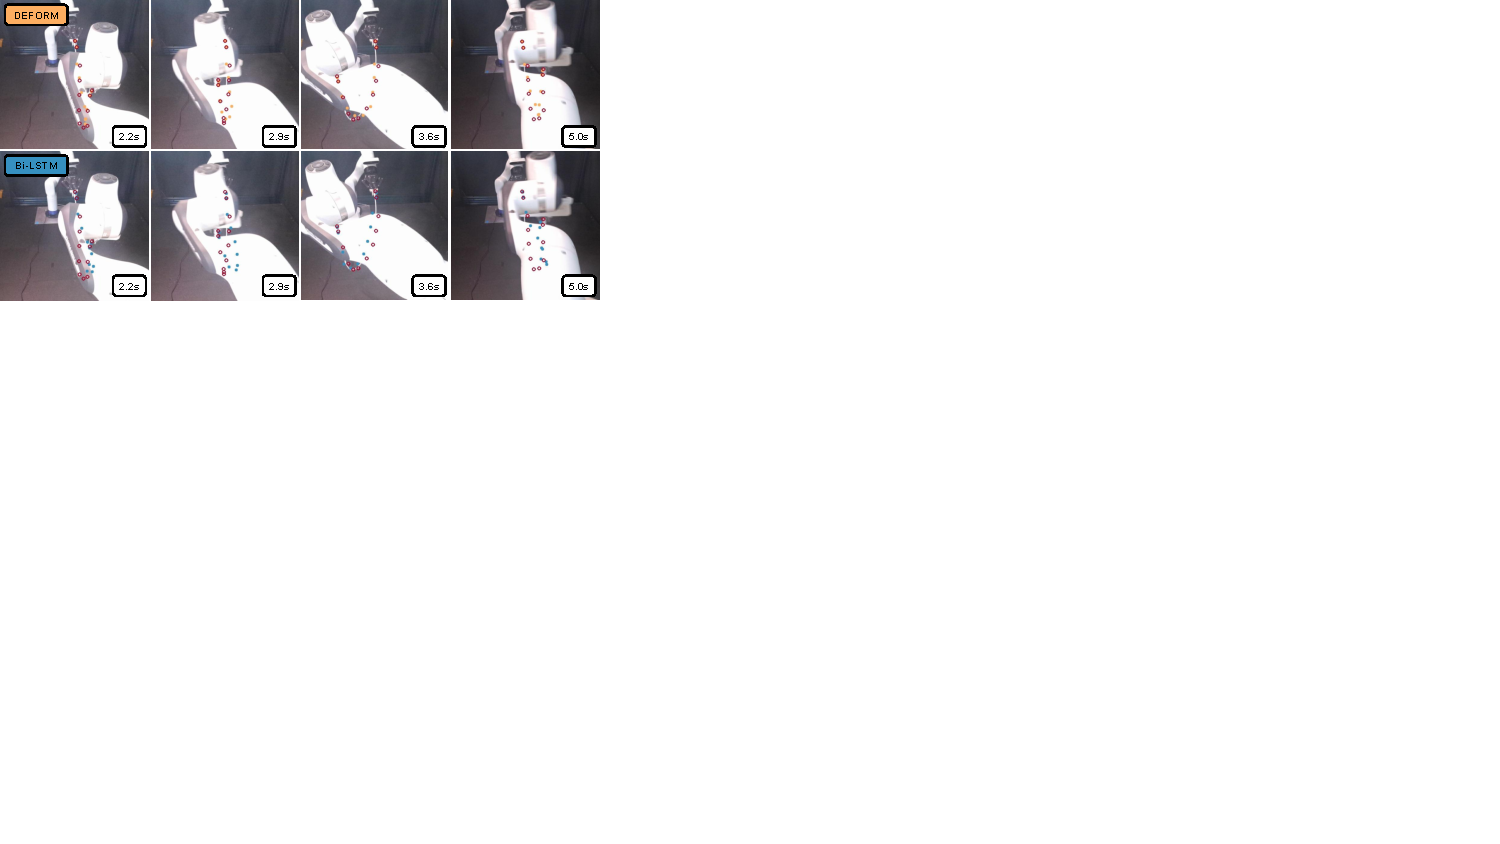
\includegraphics[width=\linewidth]{figures/exp_res_4.pdf}
        \caption{DLO 2, dual-robot manipulation}
        \label{fig:rr_thick}
    \end{subfigure}
    \vspace{-5pt}
    % % Third row
    % \begin{subfigure}{0.49\textwidth}
    %     \centering
    %     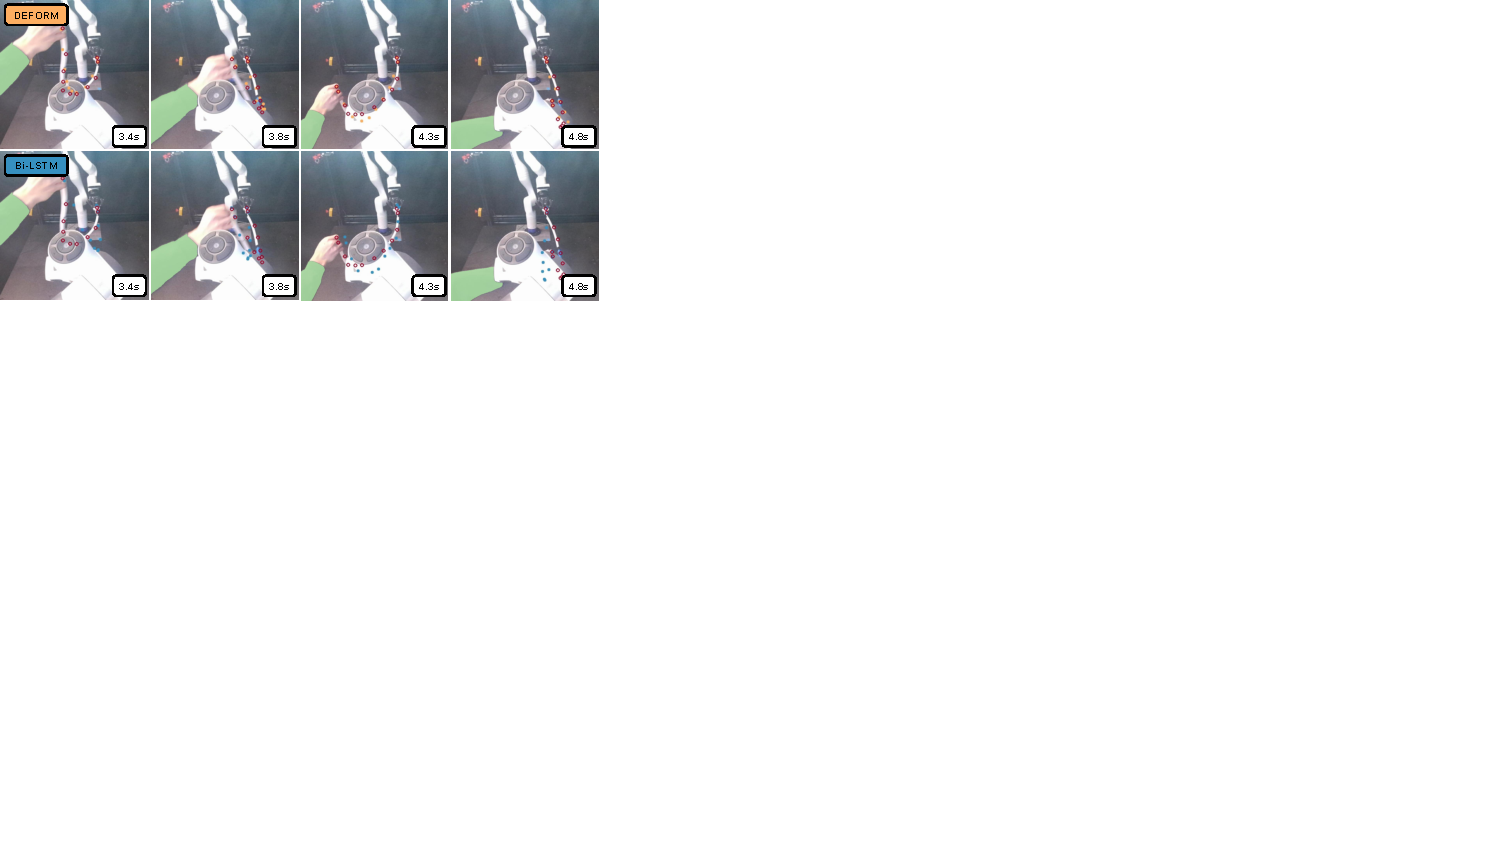
\includegraphics[width=\linewidth]{figures/exp_res_5.pdf}
    %     \caption{DLO 3, robot-human manipulation}
    %     \label{fig:rh_aniso}
    % \end{subfigure}%
    % \hfill
    % \begin{subfigure}{0.49\textwidth}
    %     \centering
    %     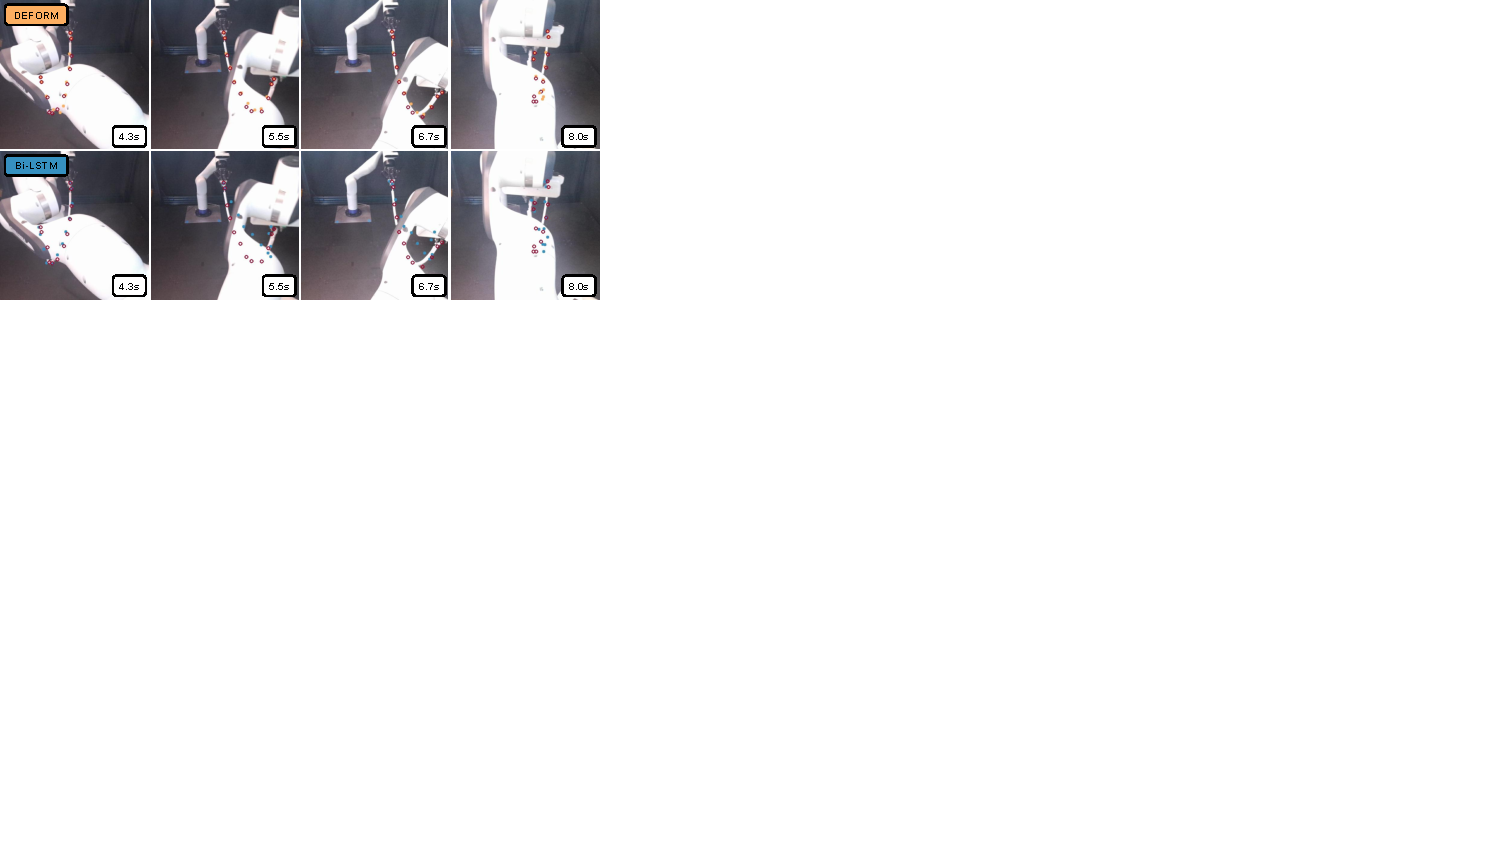
\includegraphics[width=\linewidth]{figures/exp_res_6.pdf}
    %     \caption{DLO 3, dual-robot manipulation}
    %     \label{fig:rr_aniso}
    % \end{subfigure}
    % \vspace{0.2cm}
    % \vspace{-0.2cm}

    \caption{Visualization of the performance of DEFORM and Bi-LSTM in predicting trajectories for DLOs 1 and 2. The ground truth vertices of the DLOs are marked with red hollow circles. The predicted vertices are marked with orange solid circles for DEFORM and blue solid circles for the Bi-LSTM model, respectively.}
    \label{fig:grid}
    \vspace{-13pt}
\end{figure}
\section{Experiments and Results}
\label{sec:experiments}
% \begin{figure}[t]
%     \centering
%     % First row
%     \begin{subfigure}{0.49\textwidth}
%         \centering
%         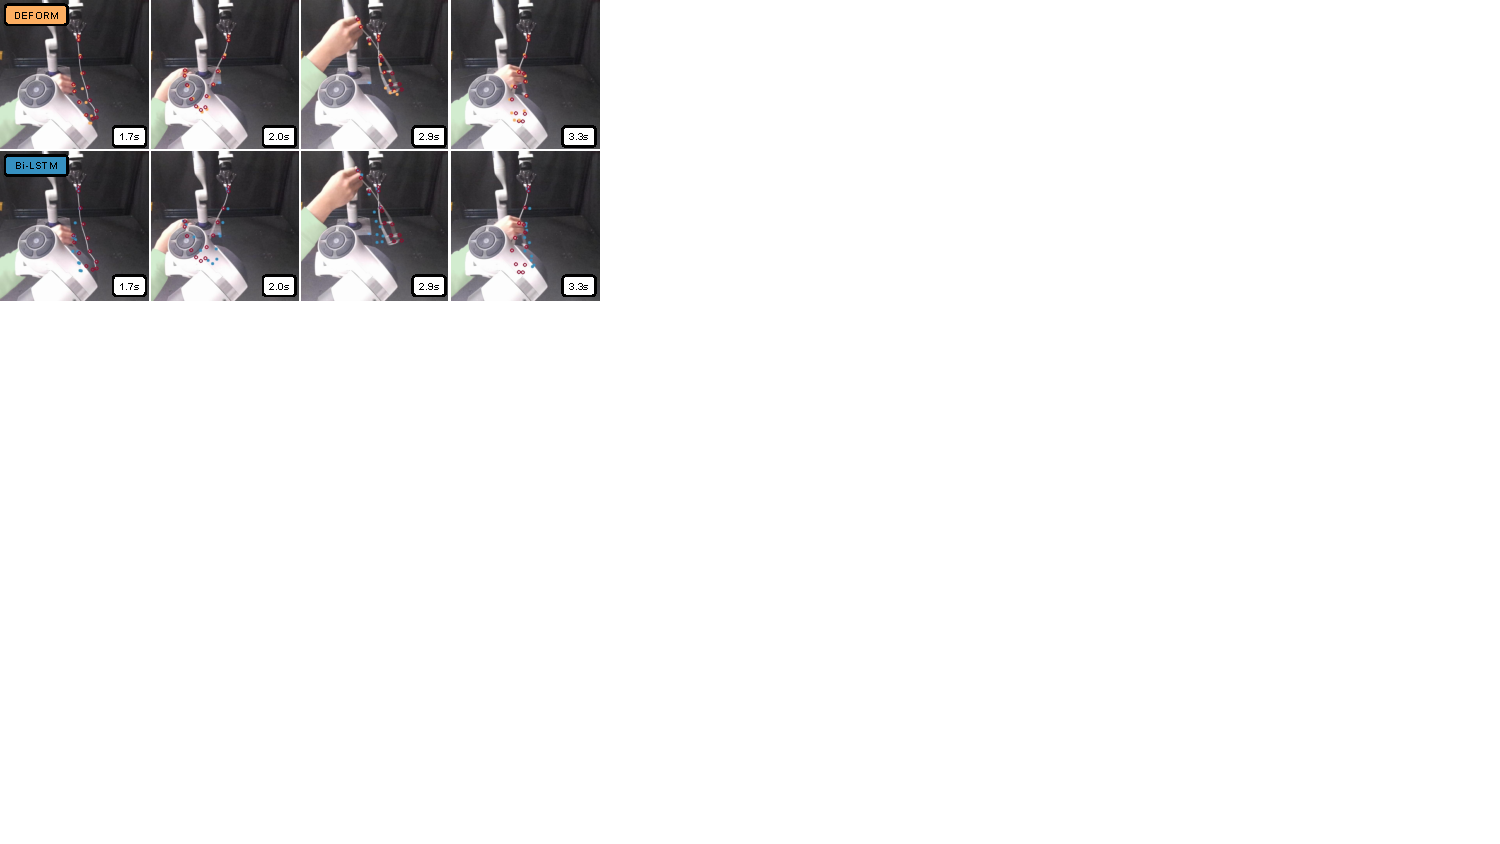
\includegraphics[width=\linewidth]{figures/exp_res_1.pdf}
%         \caption{DLO 1, robot-human manipulation}
%         \label{fig:rh_thin}
%     \end{subfigure}%
%     \hfill
%     \begin{subfigure}{0.49\textwidth}
%         \centering
%         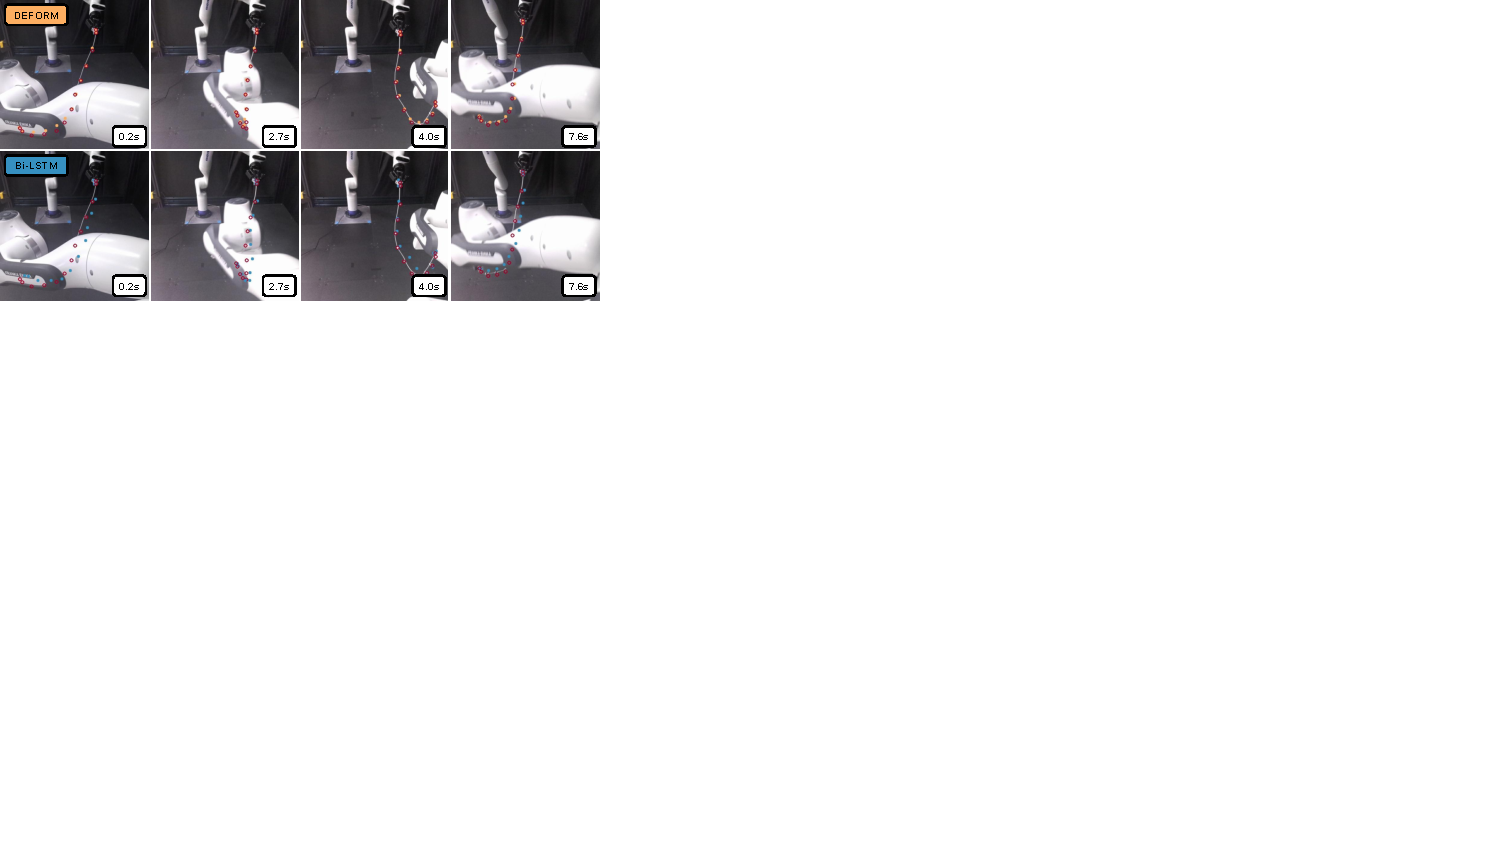
\includegraphics[width=\linewidth]{figures/exp_res_2.pdf}
%         \caption{DLO 1, dual-robot manipulation}
%         \label{fig:rr_thin}
%     \end{subfigure}
%     \vspace{-5pt}
%     \caption{Visualization of DEFORM and Bi-LSTM trajectory predictions for DLO1. DLO ground truth vertices are hollow red circles. 
%     The predicted vertices are solid orange circles for DEFORM and solid blue circles for Bi-LSTM.
%     Visualizations for DLO2 and DLO3 can be found in Appendix \ref{appendix:dlosvis}}
%     \label{fig:grid}
%     \vspace{-9pt}
% \end{figure}
This section covers the real-world evaluation of DEFORM, including: 1) a quantitative comparison of modeling accuracy with state-of-the-art methods, 2) computational speed assessment, 3) an ablation study on parameter auto-tuning, residual learning, and multi-step training, 4) using DEFORM to track DLOs with an RGB-D camera, and 5) a shape matching manipulation demonstration. 
Code and data will be provided upon final paper acceptance. 
Additional information is in Appendix \ref{appendix:Experiement Details}.
\subsection{Experiment Setup:}
% \begin{wrapfigure}{R}{0.45\textwidth} 
%     \vspace*{-0.3cm}
%     \centering
%      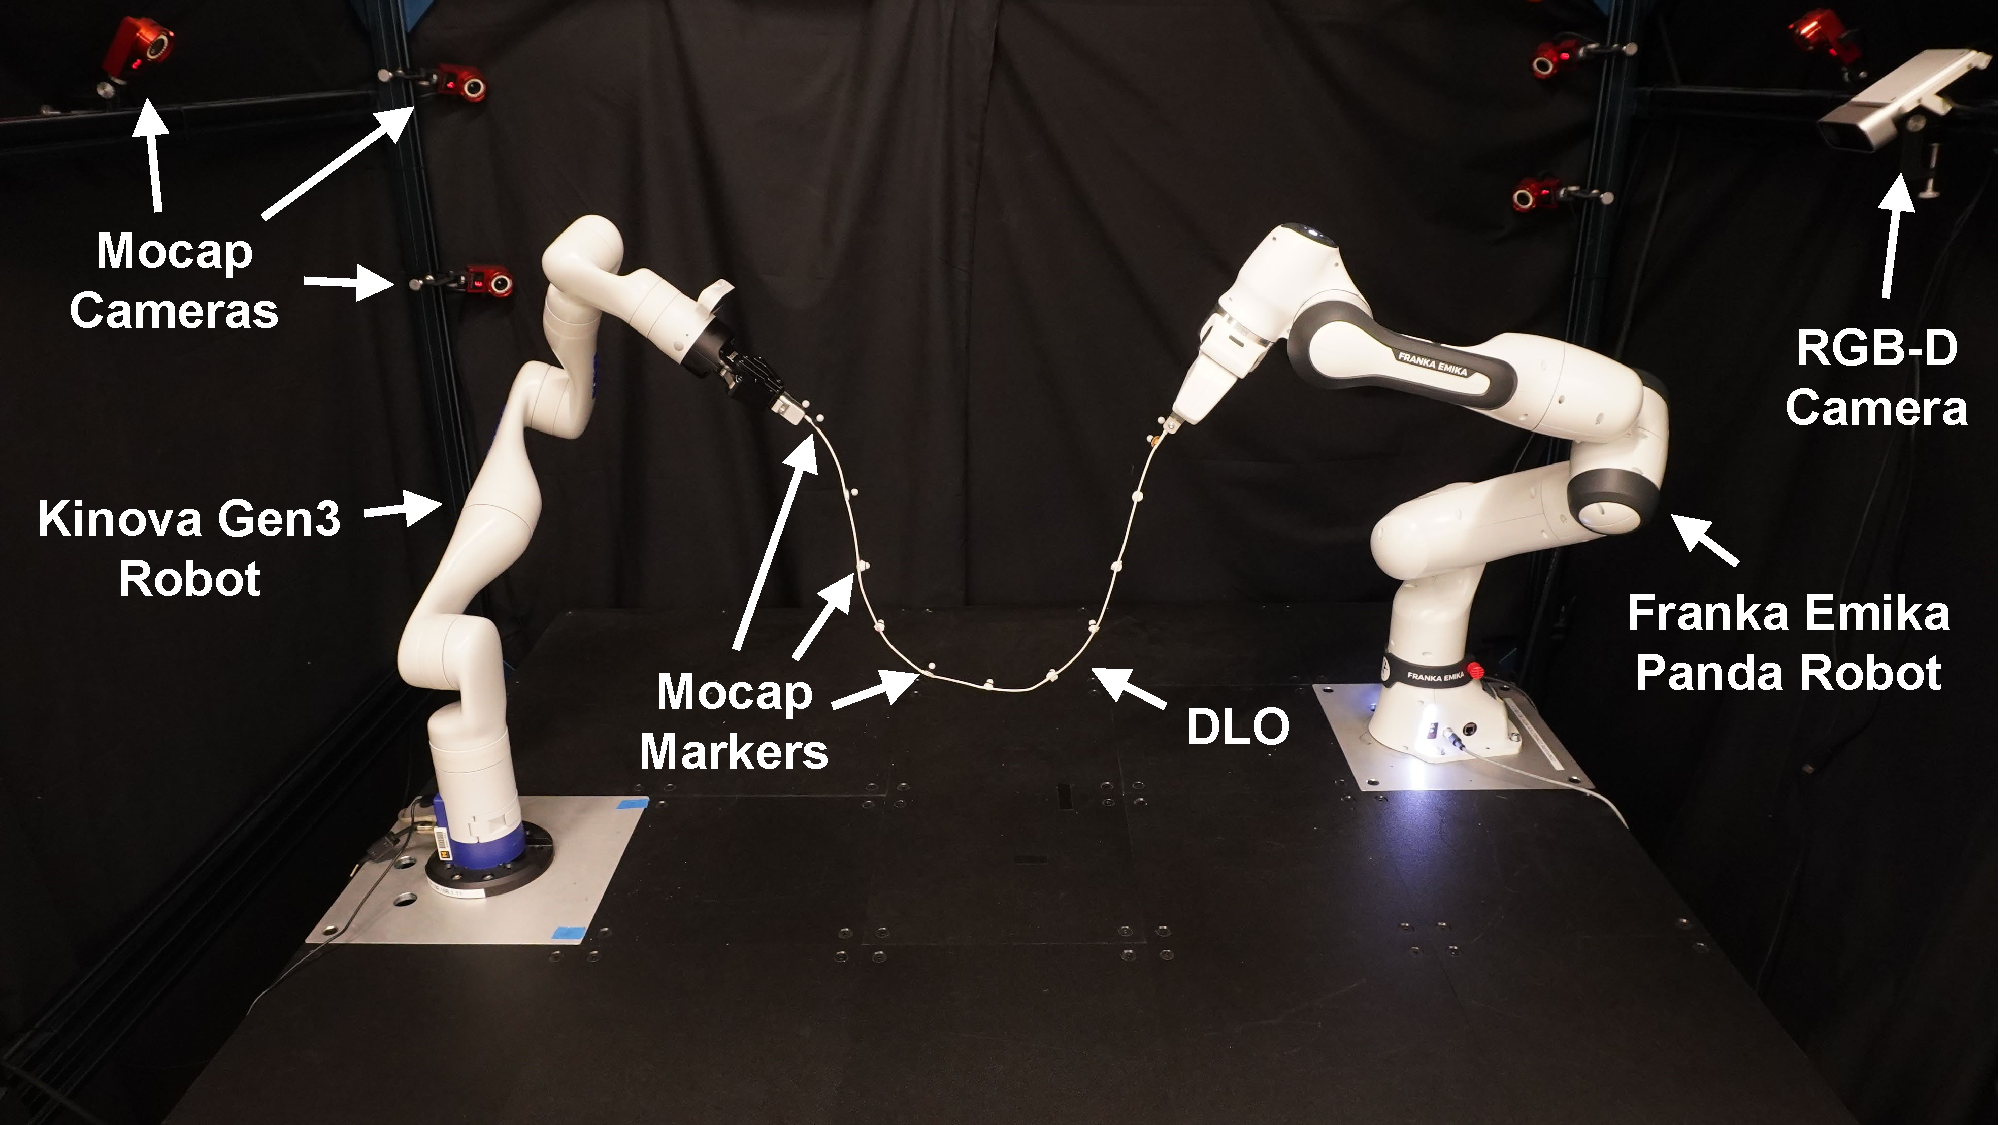
\includegraphics[width=0.45\textwidth]{figures/exp_setup_1.pdf}
%      \caption{Experiment Setup. An illustration of the experimental setup.}
%      \vspace*{-0.2cm}
%     \label{fig:exp_setup}
% \end{wrapfigure}
\textbf{Hardware Setup.}
Three distinct cables and two distinct ropes were constructed to validate the modeling accuracy of DEFORM.
Spherical markers were attached to the DLOs and are used to create training and evaluation datasets. 
We set the number of vertices equal to the number of MoCap markers. 
We use an OptiTrack motion capture (MoCap) system to obtain the ground truth vertex locations.
% \Revise{Note that the markers are used to create training and evaluation datasets, as well as evaluate the performance of DEFORM by providing the ground truth. 
% However, for real-world applications, the markers are not needed, and DEFORM only needs a depth camera for perception \Revise{}{of Section \ref{sec:perception and planning}}.}{}
% Markers are used to create training and evaluation datasets.
Because the markers are incorporated during training and evaluation, their effect on the dynamics is incorporated into all subsequent evaluations. 
Note that for real-world applications, the markers would not be needed.
A Franka Emika Research 3 robot and a Kinova Gen3 robot are used for dual manipulation. 

\textbf{Dataset Collection and Training.}
For each DLO, we collect 350 seconds of dynamic trajectory data in the real-world using the motion capture system at a frequency of 100 Hz. The model for each of the five DLOs is trained separately using the trajectory data collected from our real-world experiments.
The dataset is split with 80\% for training and 20\% for evaluation.
In training, models are trained using the same 100 steps (1s) of dynamic motion, which included slow and fast DLO motions.
% This includes a variety of different behaviors including slow and fast motions.
% This split divided the spectrum of motions evenly.
The L1 loss over the 100 step prediction horizon is used for training.
For evaluation, the trained model is used to predict DLO behavior for 500 steps without accessing ground truth.
% and a 500 step prediction horizon is used for evaluation of all models without accessing ground truth. 

% \subsection{Baseline Comparisons} 
% \begin{figure*}
%     \makebox[\textwidth][c]{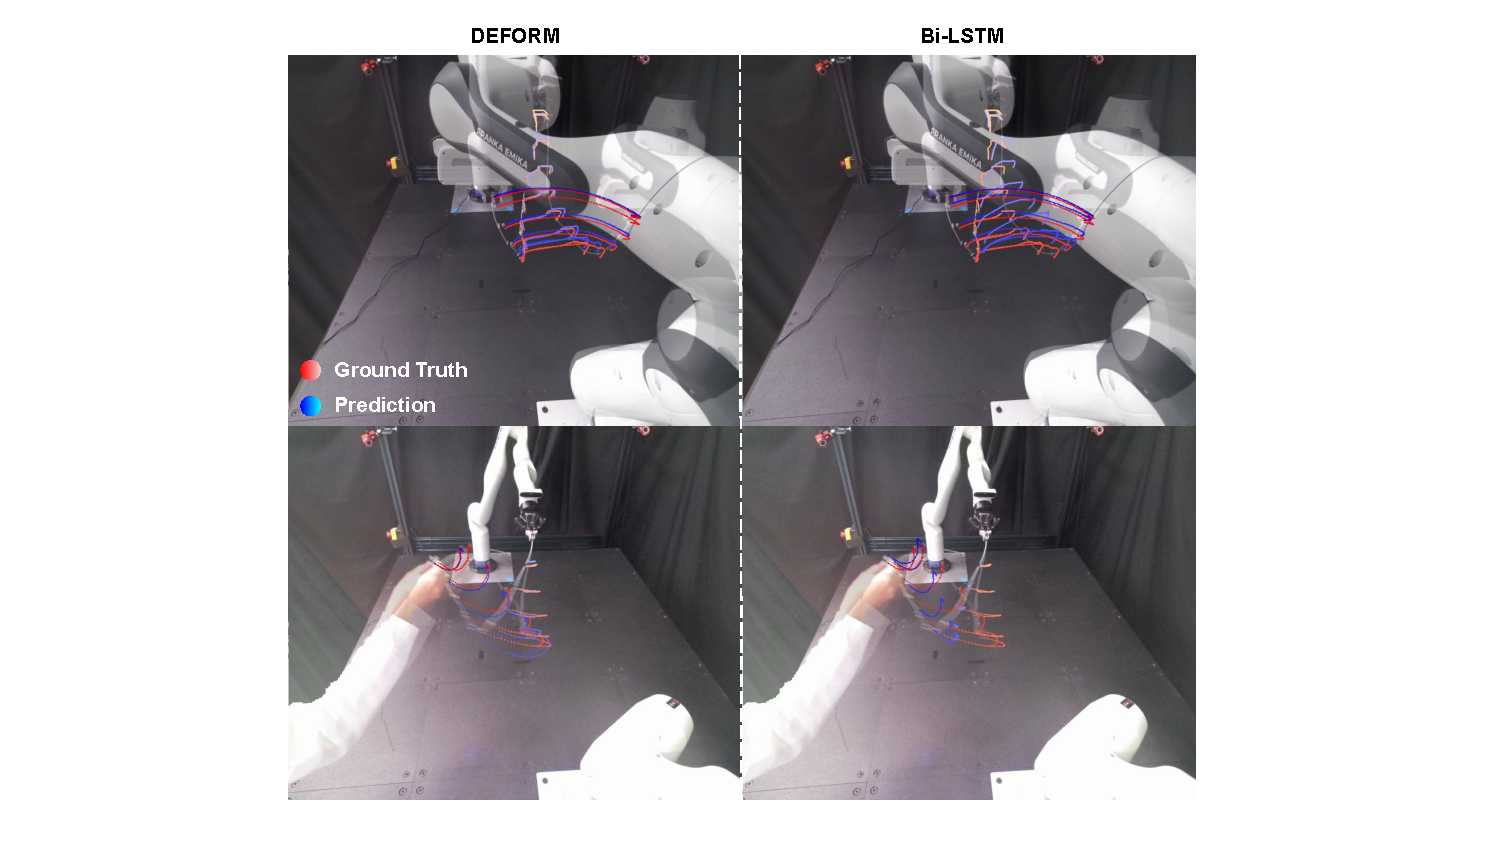
\includegraphics[width=1.7\textwidth]{figures/baseline_comp.pdf}}%
%      % \includegraphics[width=0.6\textwidth]{Copy of paper figures (3).pdf}
%      \caption{Visualization of DEFORM and Bi-LSTM on predicting two DLO trajectories. Top: Dual arm manipulation over 2.5 s; Bottom: Fast Human-Robot manipulation over 0.5s.\Yizhou{perspective}}
%     \label{fig:visualization}
% \end{figure*}
% \begin{figure}[t]
%     \centering
%     % First row
%     \begin{subfigure}{0.49\textwidth}
%         \centering
%         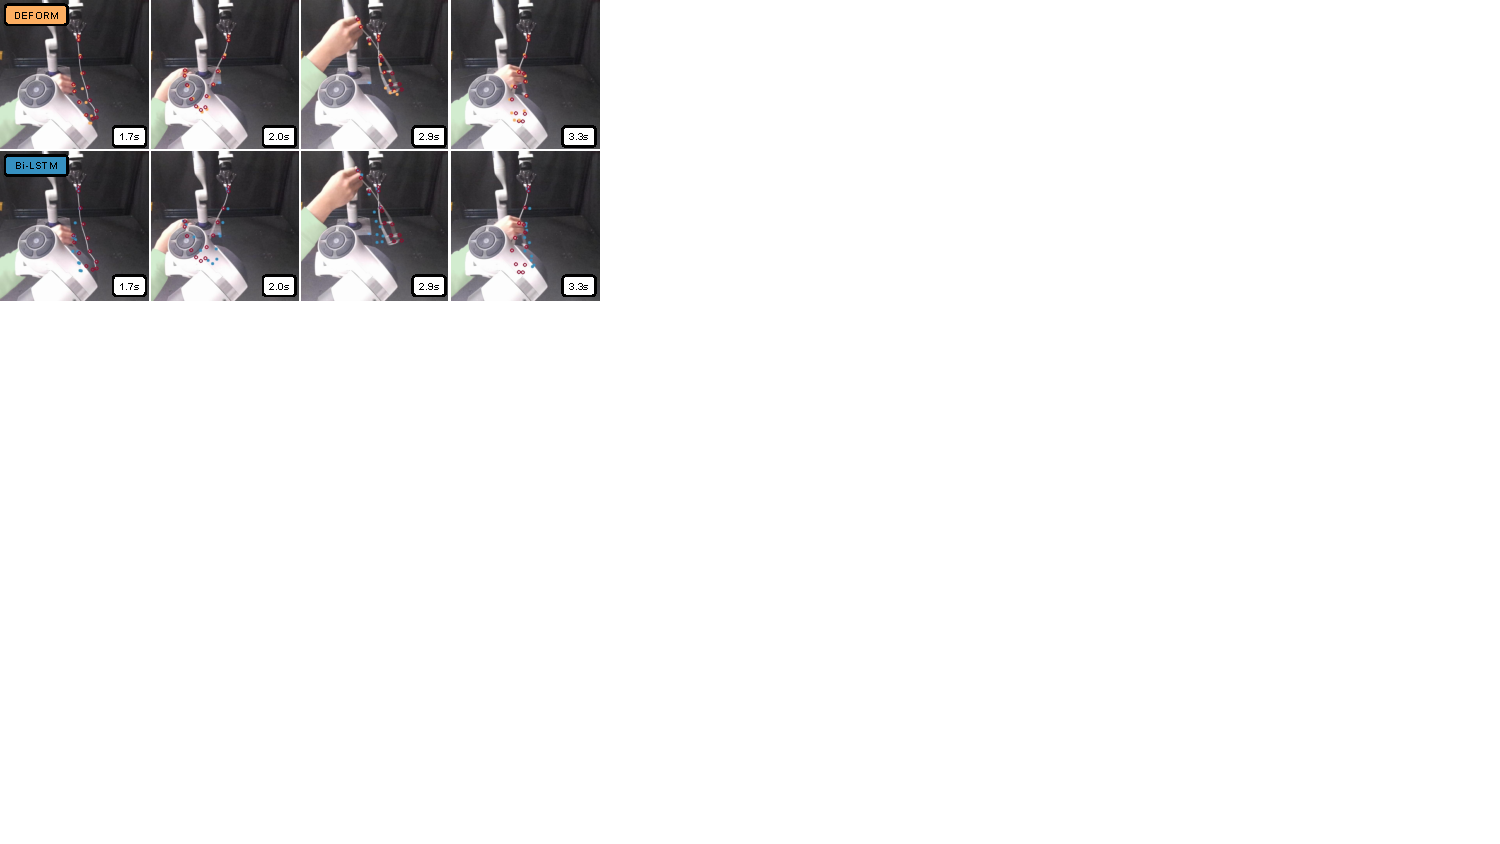
\includegraphics[width=\linewidth]{figures/exp_res_1.pdf}
%         \caption{DLO 1, robot-human manipulation}
%         \label{fig:rh_thin}
%     \end{subfigure}%
%     \hfill
%     \begin{subfigure}{0.49\textwidth}
%         \centering
%         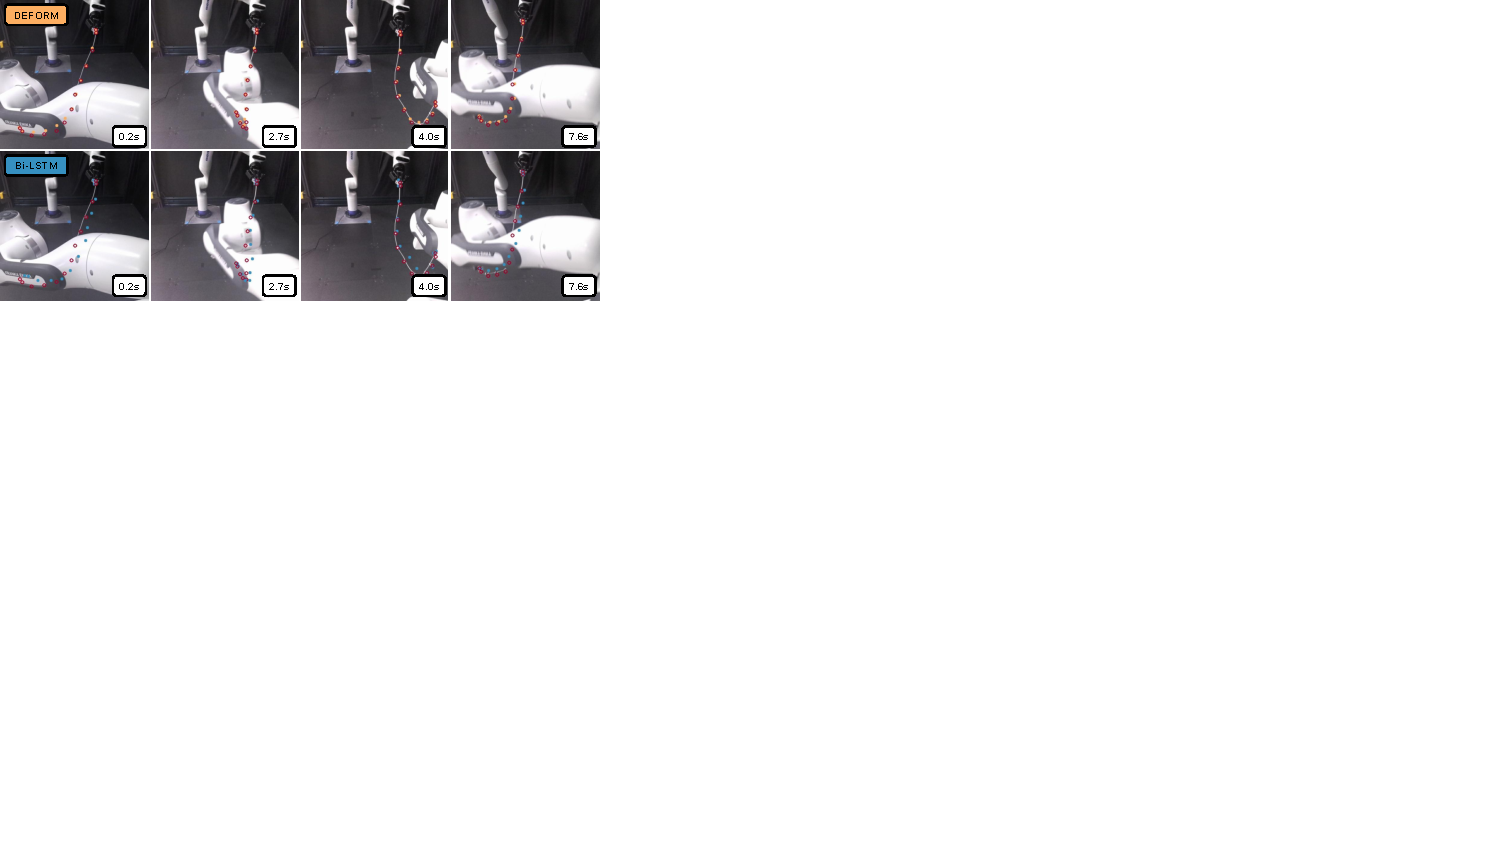
\includegraphics[width=\linewidth]{figures/exp_res_2.pdf}
%         \caption{DLO 1, dual-robot manipulation}
%         \label{fig:rr_thin}
%     \end{subfigure}
%     \vspace{0.2cm}

%     % % Second row
%     % \begin{subfigure}{0.49\textwidth}
%     %     \centering
%     %     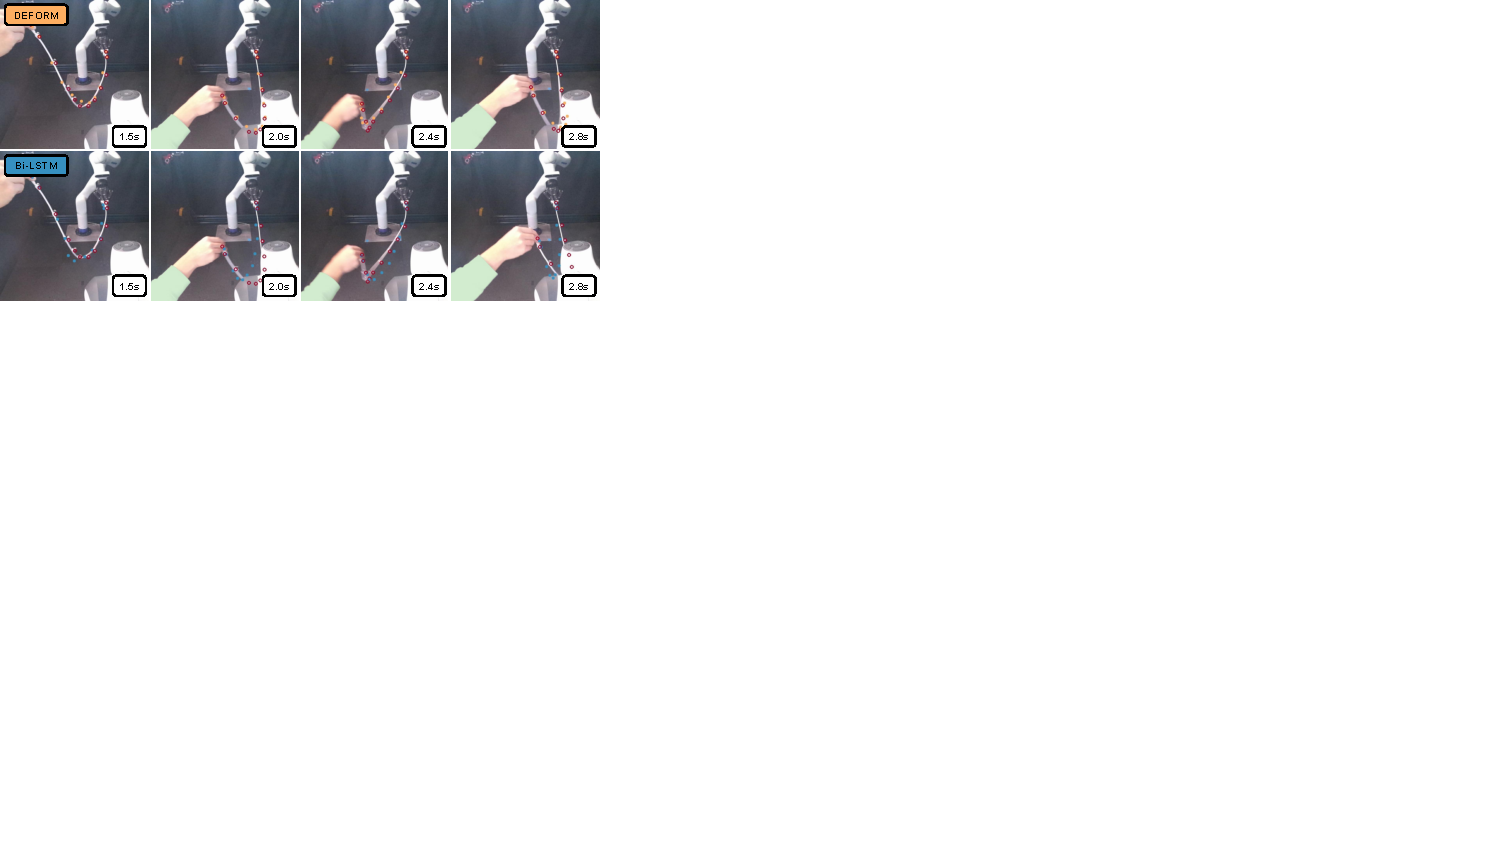
\includegraphics[width=\linewidth]{figures/exp_res_3.pdf}
%     %     \caption{DLO 2, robot-human manipulation}
%     %     \label{fig:rh_thick}
%     % \end{subfigure}%
%     % \hfill
%     % \begin{subfigure}{0.49\textwidth}
%     %     \centering
%     %     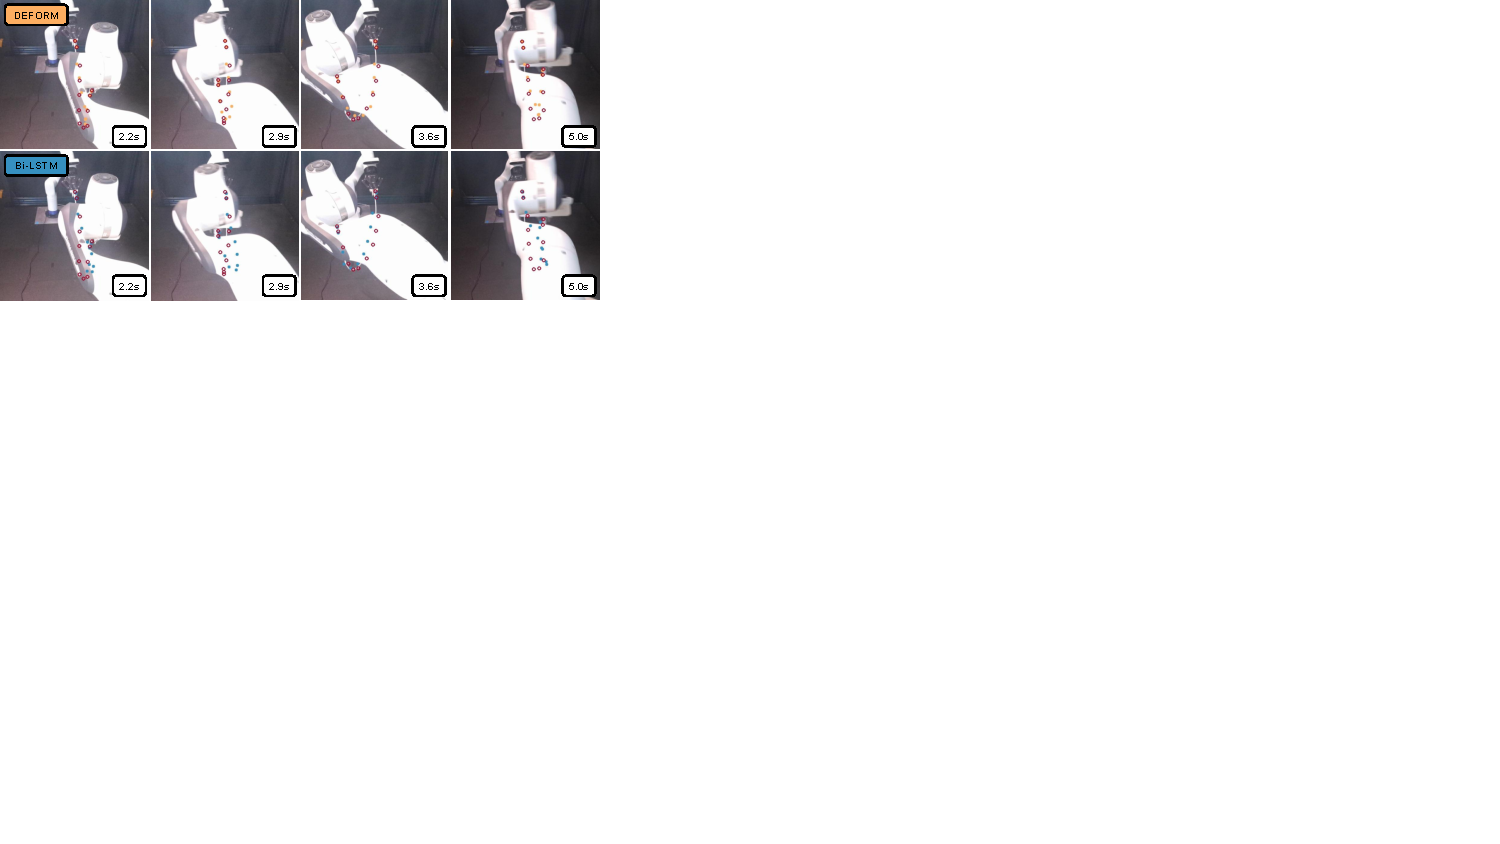
\includegraphics[width=\linewidth]{figures/exp_res_4.pdf}
%     %     \caption{DLO 2, dual-robot manipulation}
%     %     \label{fig:rr_thick}
%     % \end{subfigure}
%     % \vspace{0.2cm}

%     % % Third row
%     % \begin{subfigure}{0.49\textwidth}
%     %     \centering
%     %     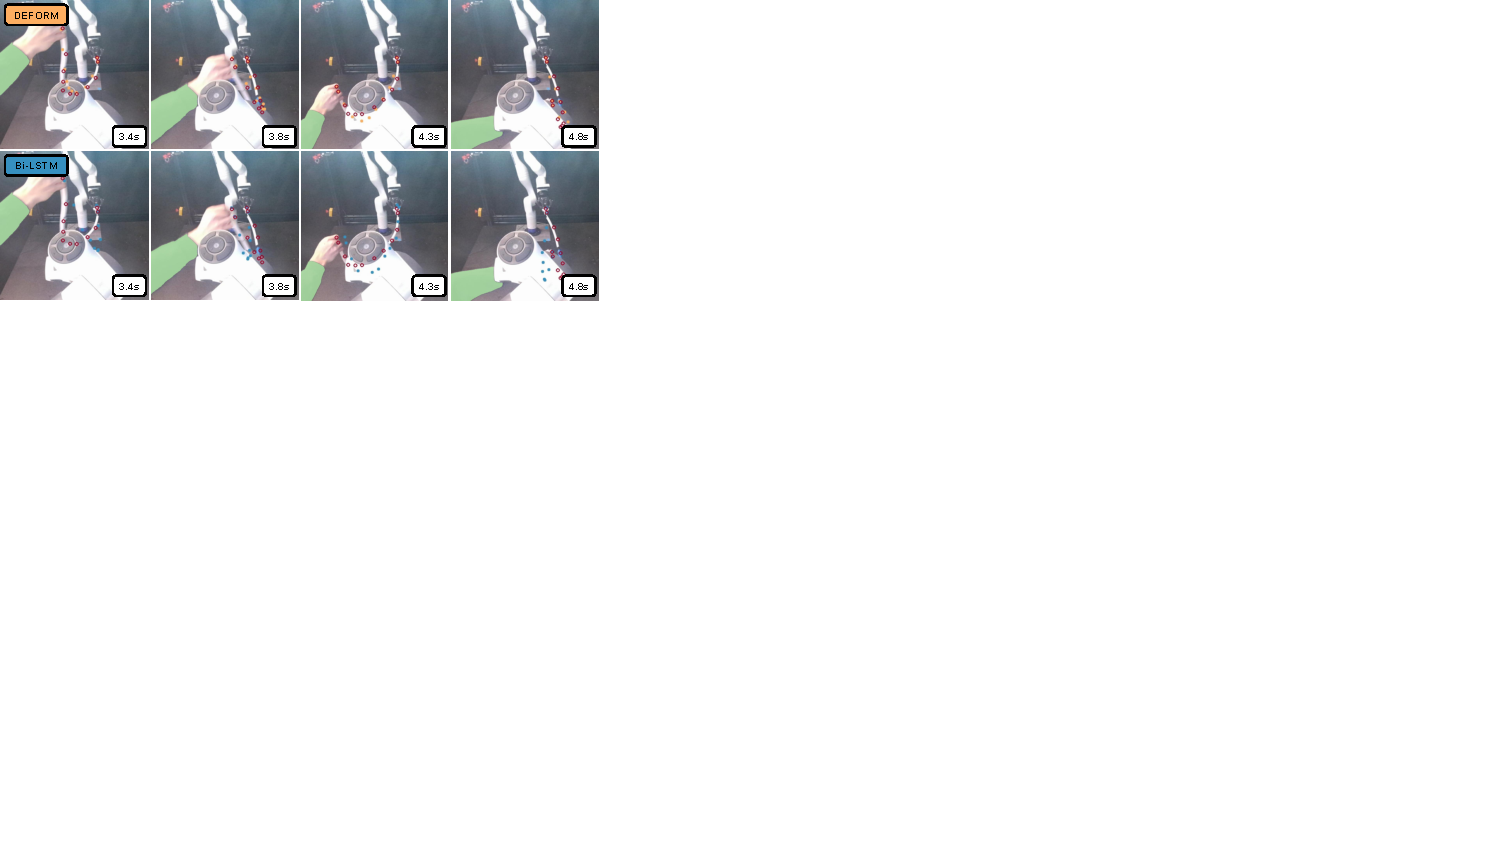
\includegraphics[width=\linewidth]{figures/exp_res_5.pdf}
%     %     \caption{DLO 3, robot-human manipulation}
%     %     \label{fig:rh_aniso}
%     % \end{subfigure}%
%     % \hfill
%     % \begin{subfigure}{0.49\textwidth}
%     %     \centering
%     %     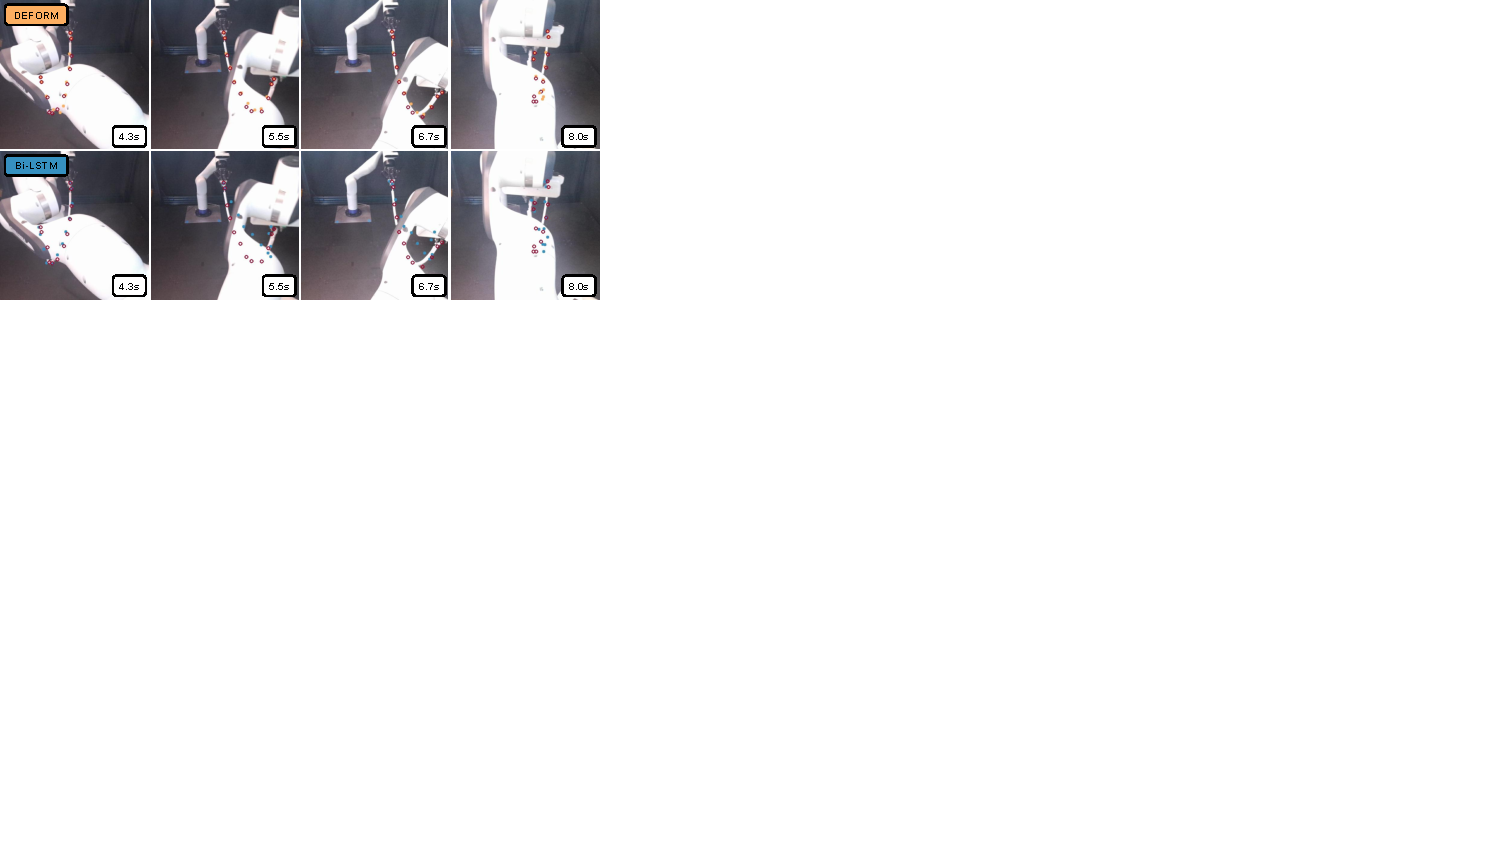
\includegraphics[width=\linewidth]{figures/exp_res_6.pdf}
%     %     \caption{DLO 3, dual-robot manipulation}
%     %     \label{fig:rr_aniso}
%     % \end{subfigure}
%     % \vspace{0.2cm}
%     % \vspace{-0.2cm}

%     \caption{Visualization of the performance of DEFORM and Bi-LSTM in predicting trajectories for DLOs 1, 2, and 3. The ground truth vertices of the DLOs are marked with red hollow circles. The predicted vertices are marked with orange solid circles for DEFORM and blue solid circles for the Bi-LSTM model, respectively.}
%     \label{fig:grid}
% \end{figure}

\textbf{Baseline Comparisons.}
\textbf{Physics-Based Modeling:} 
The XPBD~\cite{xpbd} approach is constructed using PBD, formulating constraints quasi-statically to model stretching and bending behavior.
The DRM~\cite{directionalrigidity} method is rooted in the concept of directional diminished rigidity such that the dynamics of a vertex is dependent on its configuration relative to the gripper's configuration.
% distance to the gripper while also considering the effect of the gripper's direction.
The original DER~\cite{originalDER} modeling approach is included as a baseline to demonstrate its performance when compared to other analytical methods and to DEFORM.
\textbf{Learning-Based Modeling:}
Yan et al.~\cite{bi-LSTM_baseline} and Wang et al.~\cite{GNN_baseline} use Bi-LSTM and GNN to represent a DLO and reason about interactions between the vertices respectively. 
% Wang et al.~\cite{GNN_baseline} method uses a GNN to describe the relationship among vertices to predict their behavior. 
\textbf{Physics-based models with enhancements:}
To further demonstrate the capabilities of DEFORM, we enhanced XPBD and DRM with residual learning and material property parameter tuning, which we denote as XPBD-NN and DRM-NN, respectively. 

\subsection{Modeling Results}

Table \ref{tab:model accuracy and computational speed} (\textbf{Left}) summarizes the results of using DEFORM when compared to baselines using the average L1 loss.
Performance is evaluated when predicting the state of the wire over a 5s prediction horizon.
Note that DEFORM outperforms all baselines for each of the five evaluated cables.
An illustration of the performance of these methods can be found in Figure \ref{fig:grid}.
Next, we compare computational speed for one step inference.
Table~\ref{tab:model accuracy and computational speed} (\textbf{Right}) indicates that Bi-LSTM has the fastest speed. 
Note that DEFORM is able to generate single step predictions at a 100Hz frequency. 

\vspace*{-6pt}

\begin{table*}[h]
    \centering
    \caption{\textbf{Left:} Baseline comparison results for modeling real-world DLO. \textbf{Right:} Computational Speed.}
    \begin{tabular}{l|ccccc|cccccc}
        \toprule
        & \multicolumn{5}{c|}{Modeling Accuracy ($10^{-2}$m)} & \multicolumn{5}{c}{Computational Speed ($10^{-2}$s)} \\         
        Method & 1 & 2 & 3 & 4 & 5 & 1 & 2 & 3 & 4 & 5 \\
        \midrule
        XPBD\cite{xpbd} & 4.00  & 3.85 & 3.80 & 3.62 & 4.35 & 1.45 & 1.38 & 1.33 & 1.31 & 1.36\\ 
        DRM\cite{directionalrigidity} & 3.64 & 4.16 & 3.21 & 4.02 & 4.19 & 0.45 & 0.44 & 0.43 & 0.44 & 0.41\\ 
        Bi-LSTM\cite{bi-LSTM_baseline} & 1.98 & 1.75 & 1.10 & 1.75 & 1.88 & \textbf{0.04} & \textbf{0.03} & \textbf{0.03} & \textbf{0.03} & \textbf{0.03}\\ 
        GNN\cite{GNN_baseline} & 3.41 & 2.23 &2.15 & 2.49 & 2.68 &  1.69 & 1.67 & 1.59 & 1.60 & 1.55\\
        DER\cite{originalDER} & 1.96 & 1.91 & 1.86 & 1.50 & 1.65 & 1.81 & 1.77 & 1.76 & 1.79 & 1.73\\ 
        NN-XPBD & 2.50 &  2.39  & 2.18 & 2.62 & 2.73 & 1.99 & 1.85 & 1.91 & 1.86 & 1.83\\ 
        NN-DRM & 2.91 & 3.22& 2.64  & 2.99 &  3.31 & 0.92 & 0.82 & 0.81 & 0.84 & 0.79 \\
        DEFORM & \textbf{1.01} & \textbf{0.97} & \textbf{0.77} & \textbf{0.85} & \textbf{0.99} & 0.97 & 0.92 & 0.94 & 0.95 & 0.92\\
        \bottomrule
    \end{tabular}
    \label{tab:model accuracy and computational speed}
        \vspace*{-2pt}

\end{table*}


% \Zac{this doesn't quite make sense? the w/o auto-parameter tuning is also without residual learning?} \Yizhou{w/o auto-parameter tuning is with residual learning}

\begin{wraptable}{r}{0.5\textwidth}
\centering
\vspace*{-20pt}
\caption{Ablation Study.}
\begin{tabular}{l|ccc}
        \toprule
        & \multicolumn{3}{c}{Accuracy ($10^{-2}$m)} \\         
        Method & 1 & 2 & 3  \\
        \midrule
        DER & 1.96 & 1.91 & 1.86  \\ 
        W/O Residual Learning & 1.54 & 1.77  & 1.42  \\
        W/O System ID & 1.21 &1.32& 1.09 \\ 
        Original Inextensibility & 1.65  & 1.23  & 1.00 \\
        % Residual Learning & 1.81 &1.87& 1.55  \\
        % Single-Step Training & 1.82 &1.74& 1.79  \\
        DEFORM & \textbf{1.01} & \textbf{0.97} & \textbf{0.77}  \\
        \bottomrule
        \end{tabular}
        \vspace*{-14pt}
        \label{tab:ablation study}
\end{wraptable}

\textbf{Ablation Study.}
% Next, we summarize an ablation study which demonstrates the effect of each contribution of DEFORM. 
% efficacy of our design choice. \Zac{what design choice? do you mean the effect of each contribution of the DEFORM framework?} \Yizhou{\checkmark}
Results are summarized in Table \ref{tab:ablation study} and show the effect of each DEFORM contribution.
% where a comparison to a baseline DER method is also included.
Note that a standard DER method is included as a baseline and does not include any of the DEFORM contributions.
% residual learning or employ auto-tuning of the material property parameters as was described in Section \ref{sec:Differentiable DER}.
The results of the study show that residual learning has the biggest improvement on the baseline performance, but the auto-tuning of material properties has a non-trivial affect as well. 
Further, the improved inextensibility enforcement makes a large improvement for more compliant DLOs, such as DLO1.
This is because the more compliant DLOs swing more during dynamic behavior, so ensuring momentum is conserved greatly improves prediction accuracy. 
The results for DLO4 and DLO5, as well as an additional ablation study, are in Appendix \ref{appendix:sec:addablation1} and \ref{appendix:addablation2}, respectively.
Note that the stiffnesses of the tested DLOs can be found in Appendix Table 
\ref{tab:mat_prop}.
% \Yizhou{Note that as more dynamic behavior exhibits from DLO3 to DLO1 (Stiffness of DLOs can be found in Appendix Table \ref{tab:mat_prop}), the effect on performance improvement of improved extensibility enforcement increases. It demonstrates the importance of improved extensibility enforcement while modeling dynamic behavior of DLOs.}

\textbf{State Estimation.} 
We next evaluate the performance of DEFORM when it is used in concert with
\begin{wrapfigure}[13]{r}{0.40\textwidth}
  \centering
  \vspace*{-16pt}
  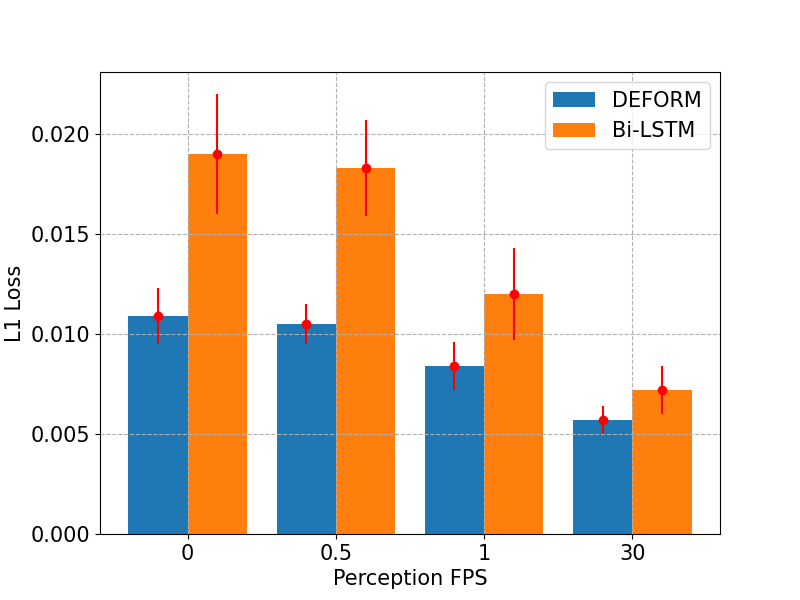
\includegraphics[width=0.45\textwidth]{figures/perception.png} 
    \vspace*{-18pt}
  \caption{The average L1 loss (m) while performing state estimation.}
  \label{fig:perception}
\end{wrapfigure} sensor observations for state estimation.
These experiments included occlusions of the DLO that arose from the manipulators or humans moving in front of the sensor. 
In this experiment, we compare how well the state estimation framework described in Appendix \ref{appendix: DLO tracking} does when using the DEFORM model versus \Revise{when using}{} the Bi-LSTM model.
Bi-LSTM was chosen because it was the second best model in terms of model accuracy. 
We also compare how well each of these methods do with varying frequencies of sensor measurement updates.
As in the earlier experiment, we evaluate the L1 norm of the prediction over a 5s long prediction horizon.
Experimental results are shown in Figure \ref{fig:perception}.
% \Revise{An illustration of the performance of these methods can be found in Figure\ref{fig:grid}.}{}
\label{sec:state estimation}
Unsurprisingly, each method improves when given access to more frequent sensor updates.
This illustrates that the state estimation algorithm described in Appendix \ref{sec:tracking} behaves appropriately.
Notably, the DEFORM model with no state estimation does better than the Bi-LSTM model even when the Bi-LSTM model is given access to 1 fps updates. 
The method using the DEFORM model with access to 30 fps sensor measurements is the most effective.

\textbf{3-D Shape Matching Manipulation.}
\begin{figure}[t]
    \centering
     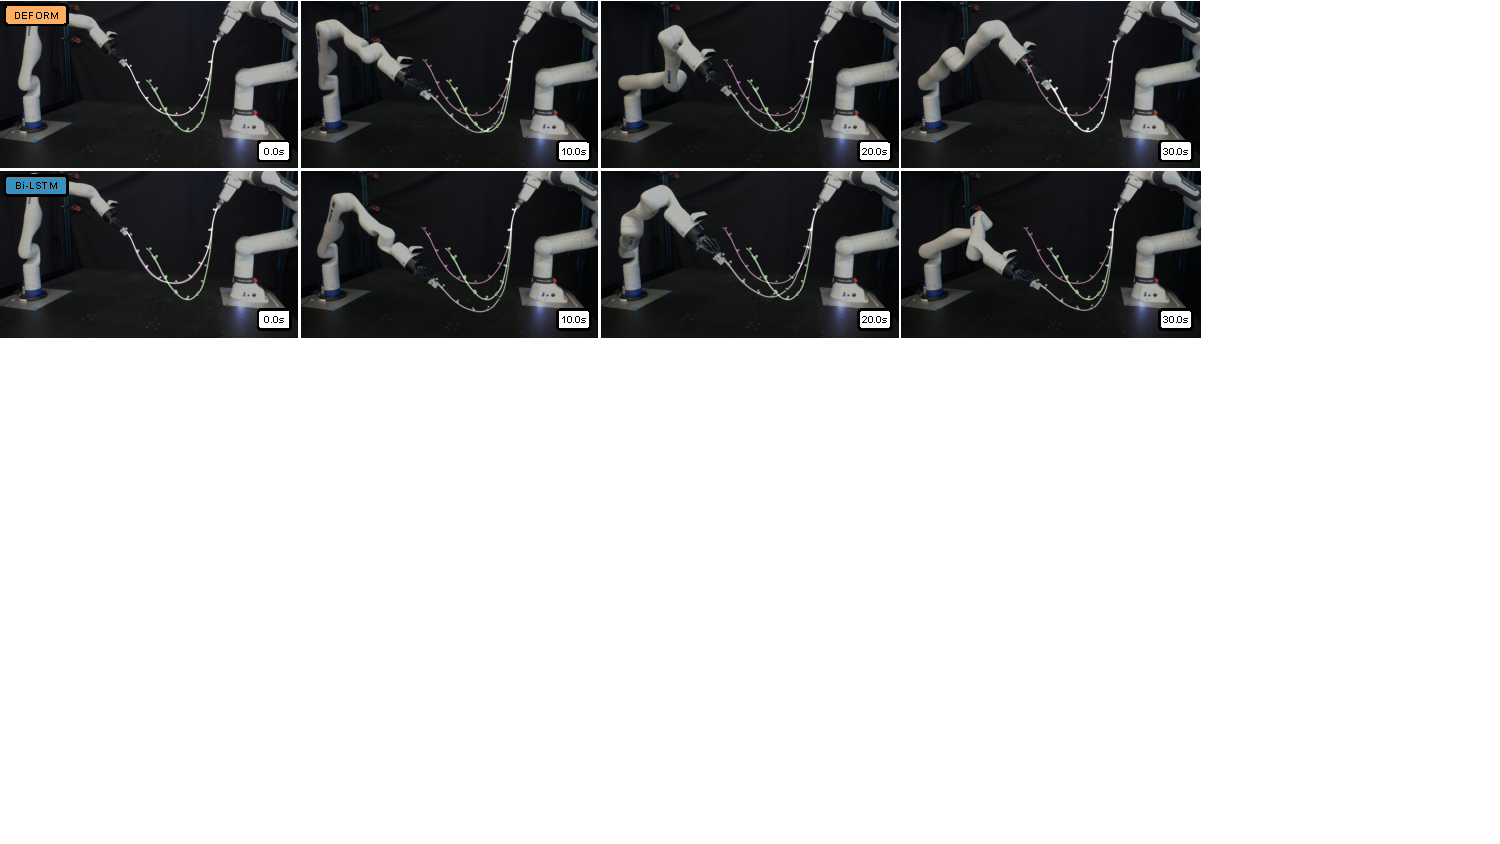
\includegraphics[width=1\textwidth]{figures/shape_control_exp.pdf}
     \caption{A time lapse comparison of the DEFORM model and the Bi-LSTM model when each is used to perform a shape matching task. 
     The goal configuration is green whereas the start configuration is pink. 
     The DEFORM model enables the planning algorithm to successfully complete the task whereas the planning algorithm using the Bi-LSTM model fails to complete the task.}
    \label{fig:shape_control_exp}
    \vspace*{-16pt}
\end{figure}
To demonstrate the practical applicability of DEFORM, we illustrate its use for DLO 3-D shape matching tasks in both simulation and the real world.
\begin{wraptable}{r}{0.35\textwidth}
    \vspace*{-0.25cm}
    \centering
\caption{Shape matching manipulation success rate}
    \begin{tabular}{l|cc}
        \toprule         
        & \multicolumn{2}{c}{Success Rate} \\         
        Method & Real & Sim \\
        \midrule
        Bi-LSTM & 10/20 & 78/100 \\ 
        DEFORM & \textbf{17/20} & \textbf{90/100} \\  
        \bottomrule
    \end{tabular}
\label{tab:manipulation}
    \vspace*{-0.25cm}

\end{wraptable}
This experiment uses ARMOUR \cite{ARMOUR}, a receding-horizon trajectory planner and tracking controller framework, to manipulate DLOs. 
ARMOUR uses either DEFORM or Bi-LSTM to predict the manipulated DLO state and tries to match the final DLO configuration with a desired configuration.
% In this evaluation, we compare the performance of DEFORM and Bi-LSTM when each is used to predict the state of the DLO while following the trajectory chosen by ARMOUR, a receding-horizon trajectory planner and tracking controller framework designed for robotic manipulators. 
Details of combining ARMOUR with the DLO simulators are in Appendix \ref{appendix ARMOUR}.
We compare the performance of each method on 100 random cases in a PyBullet simulation and 20 random cases in the real world. 
% Each case features a unique combination of initial and target DLO configurations. 
If the Euclidean distance between each individual pair of ground truth and desired DLO vertices is less than 0.05 meters, then the trial is a success.
ARMOUR is given 30 seconds to complete the task, otherwise the trial is marked as a failure. 
The results are summarized in Table~\ref{tab:manipulation} and Figure \ref{fig:shape_control_exp} shows one of the real-world results.
% An illustration of the results of this comparison experiment can be found in Figure \ref{fig:shape_control_exp}.
A video of these experiments can be found in the supplementary material.
\vspace*{-0.25cm}



